\section{Methods}
\label{sec:4.4_methods}


% 4.4.1
% -----
\subsection{Tissue and sample preparation}
\label{sec:4methods_prep}

\subsubsection{Rat pancreas}
\label{sec:4methods_prep_rp}
Fresh pancreas from an 83 day old rat was cut into small pieces and fixed in 4\% paraformaldehyde (PFA, Merck) + 0.1\% glutaraldehyde (GA; Polysciences) as described in \textcite{ravelli2013destruction}. The sample was post-fixed in 1\% osmium tetroxide and 1.5\% potassium ferrocyanide in \SI{0.1}{M} cacodylate buffer, dehydrated through ethanol series and embedded in EPON (Serva). \SI{100}{\nano\meter} sections were cut and placed onto ITO-coated glass coverslips (Optics Balzers). Immunolabeling was performed as described previously \cite{kuipers2015scanning}. Samples were etched with 0.1\% periodic acid for 10 min, followed by a \SI{30}{\minute} blocking step: 1\% bovine serum albumin (BSA; Sanquin, Netherlands) in tris-buffered saline (TBS), pH 7.4. Next, anti-insulin was incubated for \SI{2}{\hour} (guinea pig; 1:50, Invitrogen, PA1-26938, RRID: AB\_794668) followed by washing and subsequent incubation for \SI{1}{\hour} with biotinylated secondary antibody (donkey-anti-guinea pig; 1:400, Jackson Immunoresearch) followed by washing steps. Finally, streptavidin conjugated AF594 (1:100, Jackson Immunoresearch) were incubated for \SI{1}{\hour} followed by washing a \SI{10}{\minute} incubation with Hoechst and washing.

\subsubsection{Mouse breast tumor cells}
\label{sec:4methods_prep_mbtc}
Mice were fixed by vascular perfusion with 4\% formaldehyde (FA) in \SI{0.1}{M} phosphate buffer (\SI{1.5}{\milli\liter\per\minute}) for ${\sim}$\SI{5}{\minute} until organs and eyes are clearly discolored. Tumors were dissected and cut immediately in blocks (${\sim}$\SI{1}{\milli\meter^3}) in 4\% FA fixative at room temperature. 4\% FA immersion fixation for \SI{3}{\hour} at room temp was continued with 2\% PFA + 2.5\% GA immersion fixation for \SI{2}{\hour} at room temperature, and the samples were stored in glass vials with 4\% FA until further processed. Samples were postfixed with 1\% osmium tetroxide and 1.5\% potassium ferrocyanide in \SI{0.065}{M} phosphate buffer for \SI{2}{\hour} at \SI{4}{\celsius} and finally for \SI{1}{\hour} with 0.5\% uranyl acetate. Dehydration was performed using a graded ethanol series. Samples were embedded in EPON resin (EMbed 812, EMS) and polymerized for \SIrange{48}{60}{\hour} at \SI{65}{\celsius}. Ultrathin section of \SI{100}{\nano\meter} were cut using a microtome (Leica, UC6) and placed on ITO glass. Hoechst 33258 (Sigma) staining was performed for \SI{120}{\minute} followed by a washing step with MilliQ water, and air dried.


% 4.4.2
% -----
\subsection{CLEMnet architecture}
\label{sec:4methods_architecture}

The design of CLEMnet (Figure \ref{fig:4M_architecture}) is based on U-net \cite{ronneberger2015u}, a deep CNN comprised of convolution, pooling, upsampling, and concatenation layers, designed for biomedical image segmentation. The U-net architecture was modified in several ways to make it more suitable for fluorescence predictions. The number of upsampling layers was reduced to address the resolution mismatch between EM and FM images. Additionally, the padding of images within convolution layers was removed to preserve image dimensions. Lastly, the number of convolution layers between each downsampling layer was reduced from two to one---roughly halving the number of parameters---to prevent overfitting \cite{balkenende2020clemnet}. The model architecture was developed in Tensorflow \cite{tensorflow2015-whitepaper}, an open source library for implementing machine learning models in Python, using the Keras API \cite{chollet2015keras}. All training and testing procedures were performed on NVIDIA Tesla P100 PCIe 12 GB GPU cards.

% --- Fig 4.M1 (architecture) ---
\begin{figure}[!tb]
    \centering
    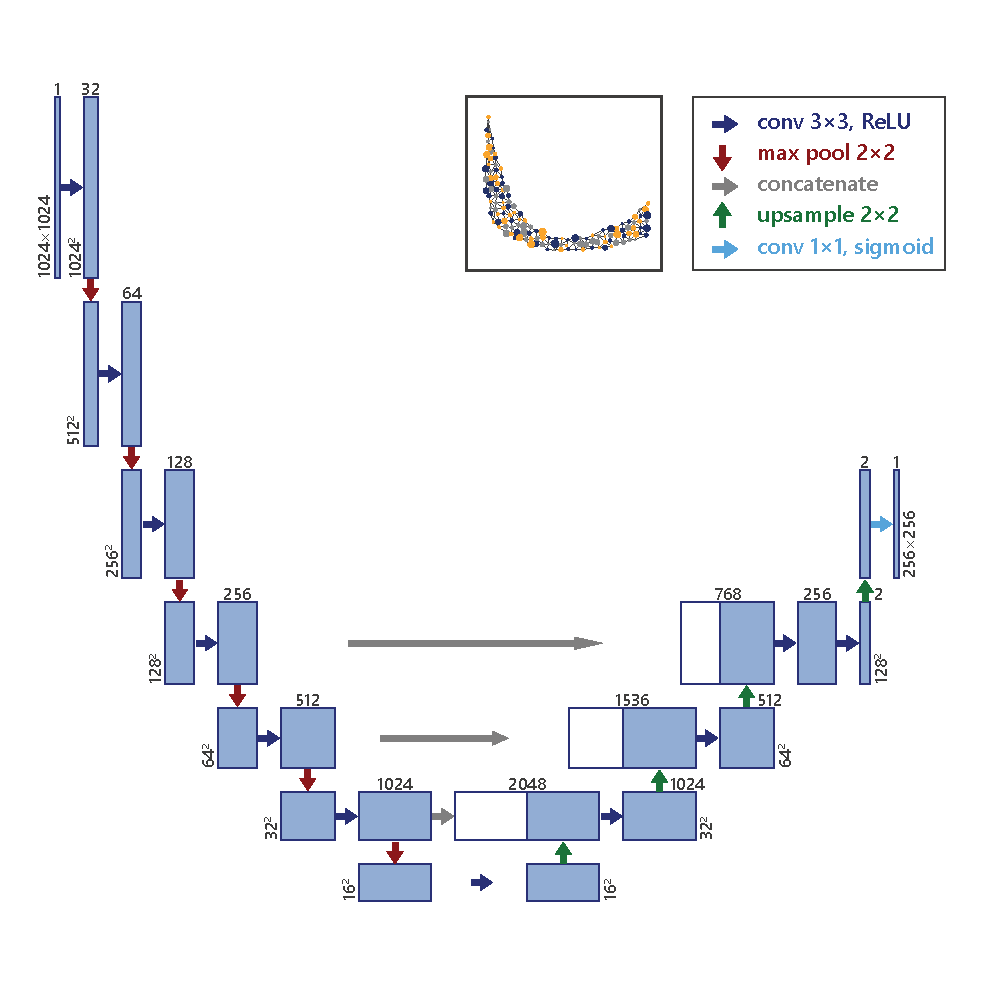
\includegraphics[width=0.95\linewidth]{chapter-4/figures_PDF/fig4-M1_architecture.pdf}
    \caption{CLEMnet architecture.
    The blue boxes correspond to multi-channel feature maps with the number of channels and image dimensions annotated above and to the side of each box, respectively. Arrows represent different possible operations as described in the legend. The asymmetric layout underlies the illustration from Figure \ref{fig:4.1_overview}B.}
    \label{fig:4M_architecture}
\end{figure}


% 4.4.3
% -----
\subsection{Data acquisition}
\label{sec:4methods_acquisition}
The integrated microscopy workflow for large-scale correlative imaging and reconstruction is described in \textcite{lane2022integrated}. Briefly, fluorescence imaging is done via the Delmic SECOM (Delmic B.V.), which has been retrofitted into the vacuum chamber of a Verios 460 SEM (Thermo Fisher Scientific) \cite{liv2013simultaneous, zonnevylle2013integration}. Correlative FM and low-magnification EM image tiles are acquired in a grid-like pattern encompassing each tissue section. The fluorescence is captured prior to EM to avoid quenching of the fluorescence. Following the acquisition of each correlative image pair, the FM tile is registered to the low-magnification EM tile by means of cathodoluminescent markers \cite{haring2017automated}. The fluorescence signal is then used to guide to regions of interest for subsequent, high-magnification EM, such as the islet of Langerhans in the case of the rat pancreas tissue. As thin sections of the mouse breast tumor cells are more or less homogeneous, acquisition areas were chosen based on minimal damage to the section. 

Each FM tile consists of a \SI{10}{\second} exposure at \SI{405}{\nano\meter} excitation for Hoechst and \SI{555}{\nano\meter} excitation for AF594. The corresponding low-magnification EM tiles are acquired at \SI{1.5}{\kilo\electronvolt} landing energy with a \SI{1}{\kilo\volt} bias potential, as described in \textcite{lane2021optimization}, with a \SI{400}{\pico\ampere} primary beam current, \SI{5}{\micro\second} dwell, and \SI{150}{\micro\meter} field width. The baseline imaging parameters for high magnification EM are the same as those for low-magnification EM with the exception of a \SI{2}{\micro\second} dwell and \SI{12}{\micro\meter} field width (${\sim}$\SI{3}{\nano\meter} pixel size). Imaging parameters for the datasets of mouse breast tumor cells acquired to assess network robustness are provided in Table \ref{tab:4M_params}. All of the image data used in this work is publicly available.\footnote{\href{https://sonic.tnw.tudelft.nl/catmaid/}{https://sonic.tnw.tudelft.nl/catmaid/}} Visualization and navigation of the large-scale datasets is made possible by CATMAID \cite{saalfeld2009catmaid}.

% --- Table 4.1 (params) ---
\begin{table}[tbh]
    \centering
    \small
    \begin{tabular}
        {>{\raggedleft\arraybackslash}p{0.8cm} % Z
         >{\raggedleft\arraybackslash}p{2cm} % Section
         >{\raggedleft\arraybackslash}p{1cm} % LE
         >{\raggedleft\arraybackslash}p{1cm} % Dwell
         >{\raggedleft\arraybackslash}p{1cm} % PS
         >{\raggedleft\arraybackslash}p{1cm} % N
         >{\raggedleft\arraybackslash}p{1.5cm} % A
         >{\raggedleft\arraybackslash}p{1cm} % T
        }
        \toprule
        Z & Section ID & LE (eV) & Dwell (µs) & Pixelsize (nm) & N. EM images & Area\quad (µm × µm) & Time (hr) \\ 
        \midrule
        10--19 & S007A--S009C & 1500 & 2 & 3 & 484 & 234 × 234 & 4.5 \\
        0 & S002A & 1500 & 3 & 3 & 484 & 234 × 234 & 6.8 \\
        1 & S003B & 1500 & 1 & 3 & 484 & 234 × 234 & 2.3 \\
        2 & S003C & 1500 & 2 & 3 & 484 & 234 × 234 & 4.5 \\
        3 & S003D & 1500 & 2 & 4 & 289 & 241 × 241 & 2.7 \\
        4 & S004A & 1500 & 2 & 5 & 196 & 249 × 249 & 1.8 \\
        5 & S004B & 1500 & 2 & 6 & 121 & 235 × 235 & 1.1 \\
        6 & S005A & 1500 & 5 & 3 & 484 & 234 × 234 & 11.3 \\
        7 & S005B & 2000 & 2 & 3 & 484 & 234 × 234 & 4.5 \\
        8 & S006A & 1000 & 2 & 3 & 484 & 234 × 234 & 4.5 \\
        9 & S006B & 3000 & 2 & 3 & 484 & 234 × 234 & 4.5 \\
        \bottomrule
    \end{tabular}
    \caption{Electron microscopy imaging settings used for the acquisition of resin-embedded mouse breast tumor cells. For data navigation purposes, Z index corresponds to section index within CATMAID.}
    \label{tab:4M_params}
\end{table}


% 4.4.4
% -----
\subsection{Robustness \& validation}
\label{sec:4methods_robustness}
EM and FM image pairs are augmented during training to increase the robustness of the model. The objective is to improve the model's flexibility and to account for different types of imaging conditions rather than to extend it to different specimens. While the model may generate reasonable predictions of the fluorescence intensity on the same cell type or organelle across different specimens, it is not generalizable to tissue or cell types it has not been trained on. Several different types of data augmentation are applied to account for the variety of imaging settings the network would reasonably encounter if tested on EM data from other instruments.

% --- Affine transformation ---
\subsubsection{Affine transformation}
Affine transformations are applied to training data such that the model learns to adapt to modest changes in structural topology. By introducing minor adjustments to the rotation ($\theta$), translation ($t_x$, $t_y$), scale ($z_x$, $z_y$), and shear ($\Gamma$) of the training data, some degree of invariance to these transformations is embedded into the model \cite{simard2003best}. The applied affine transformations are randomized for each EM-FM image pair such that each image pair receives the exact same transformation (Figure \ref{fig:4M_affine}).

% --- Fig 4.M2 (affine) ---
\begin{figure}[!tbh]
    \centering
    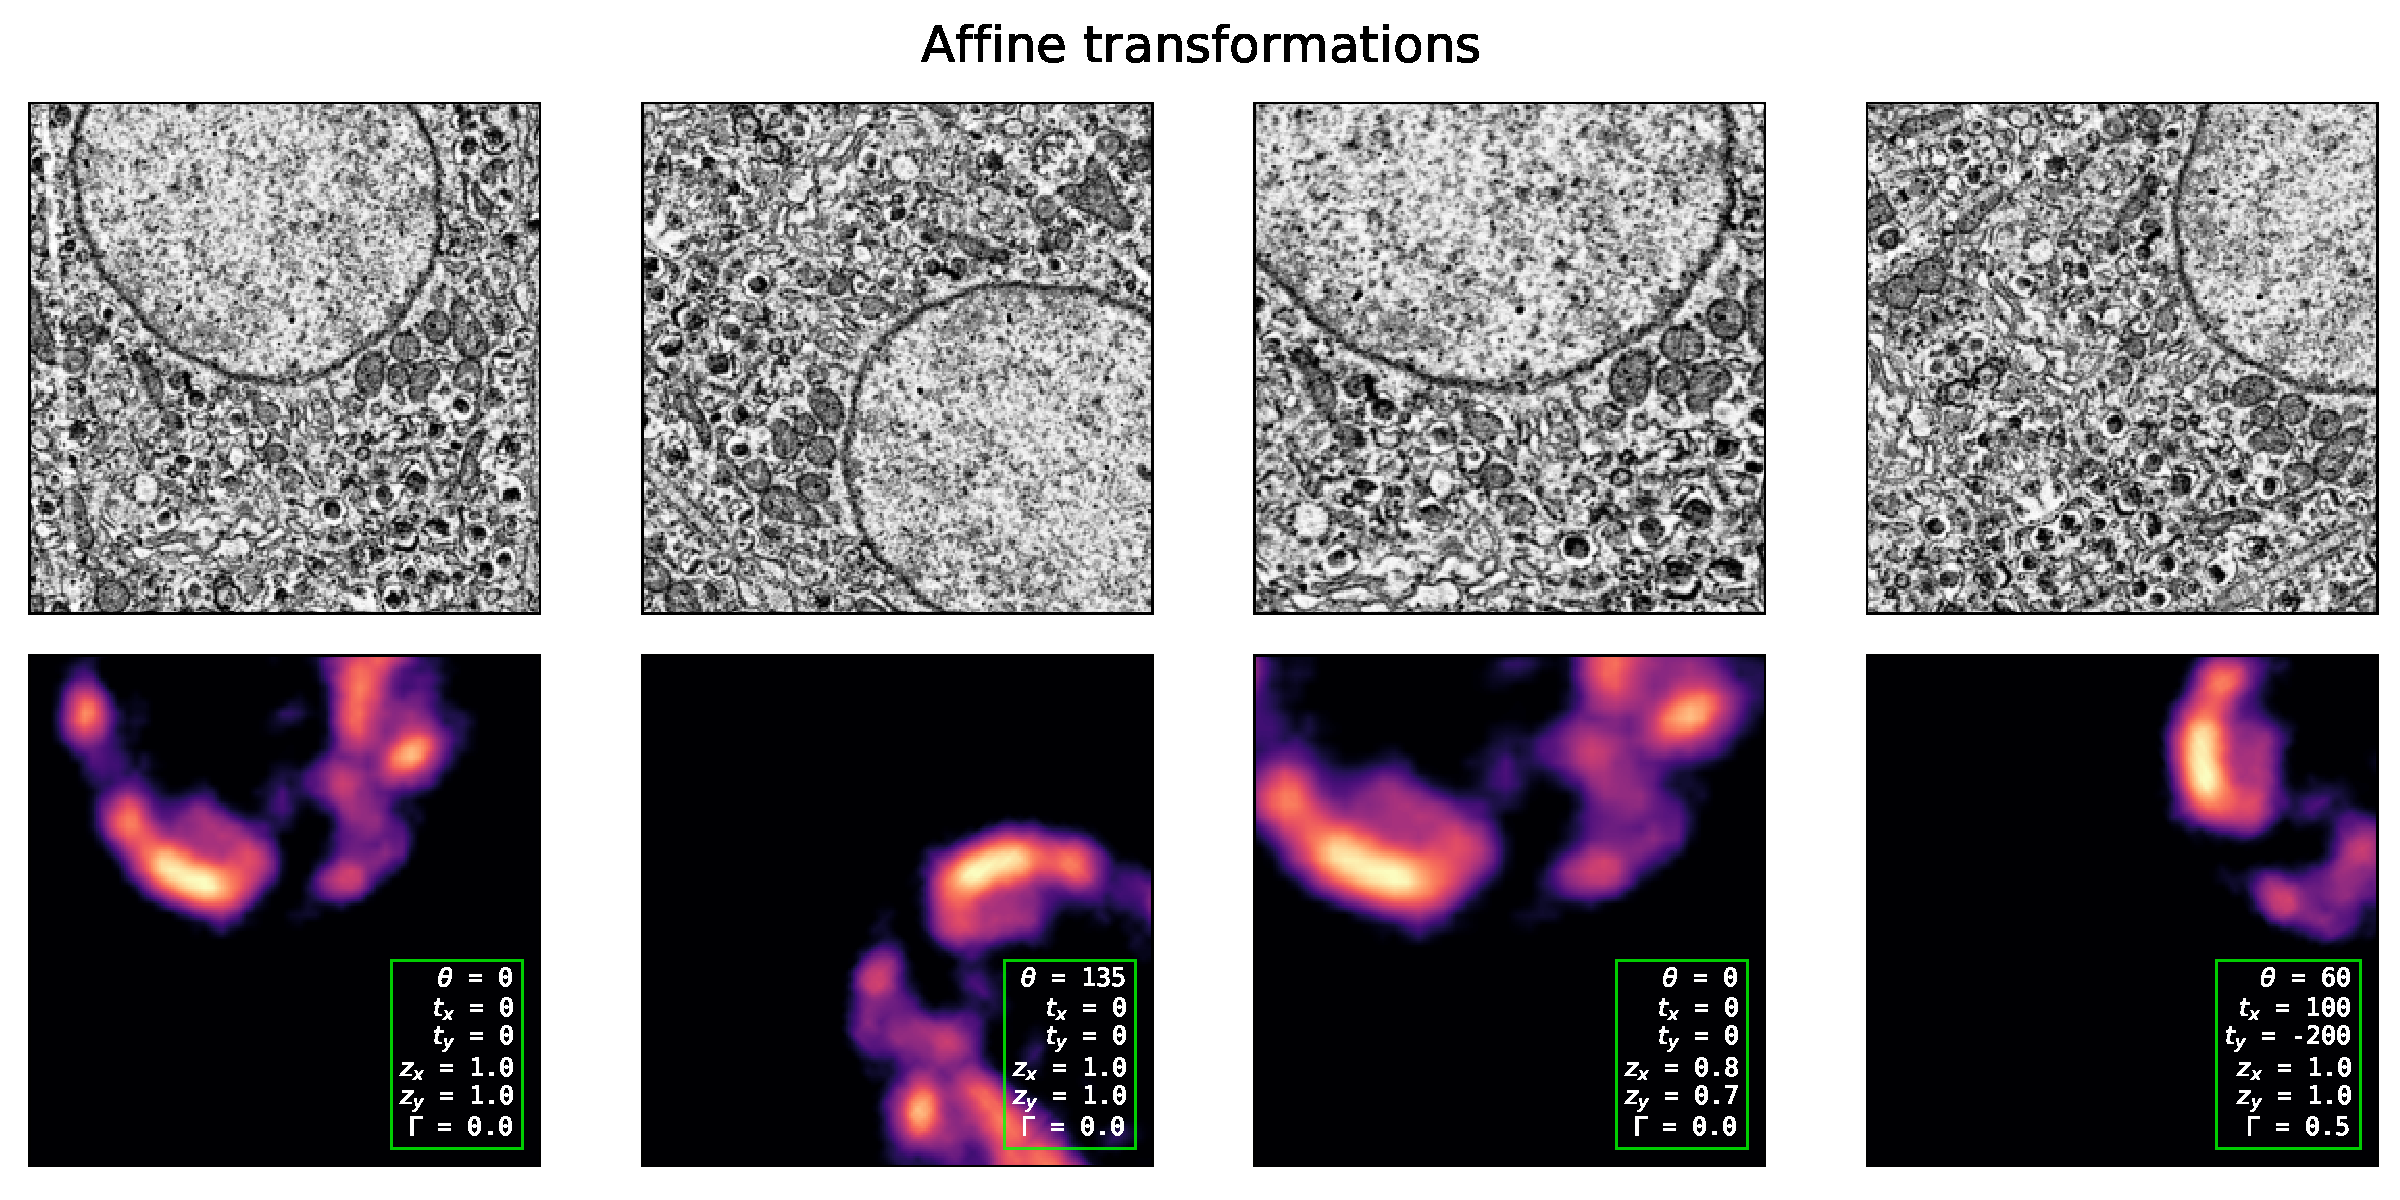
\includegraphics[width=\linewidth]{chapter-4/figures_PDF/fig4-M2_affine.pdf}
    \caption{Affine transformations are applied to the training data to render the model invariant to topological changes, resulting in greater robustness.
    The original, correlative image pair (left) may be rotated, translated, scaled, and sheared to encompass a wide variety of possible topological changes. Exact transformation parameters are provided in the text box of each transformed image pair.}
    \label{fig:4M_affine}
\end{figure}

% --- Elastic deformation ---
\subsubsection{Elastic deformation}
Elastic deformation was identified by \textcite{simard2003best} early in the development of neural networks as an effective means of augmenting training data. It was later shown by \textcite{dosovitskiy2014discriminative} and reinforced by \textcite{ronneberger2015u} as a crucial tool for enhancing CNN training, particularly in the case of limited training samples. Elastic deformations are generated by applying a non-linear warp to the image where the warp is defined by a displacement field convolved with a Gaussian kernel of standard deviation, $\sigma$, and multiplied by a scaling factor, $\alpha$ (Figure \ref{fig:4M_elastic}, top). The displacement field is initialized by a random uniform distribution where each pixel ranges from (-1, +1) with equal probability. The value for α is also randomized such that the EM images are warped with varying intensity. Distortions are more apparent along the edges of features (Figure \ref{fig:4M_elastic}, bottom).

% --- Fig 4.M3 (elastic) ---
\begin{figure}[!tb]
    \centering
    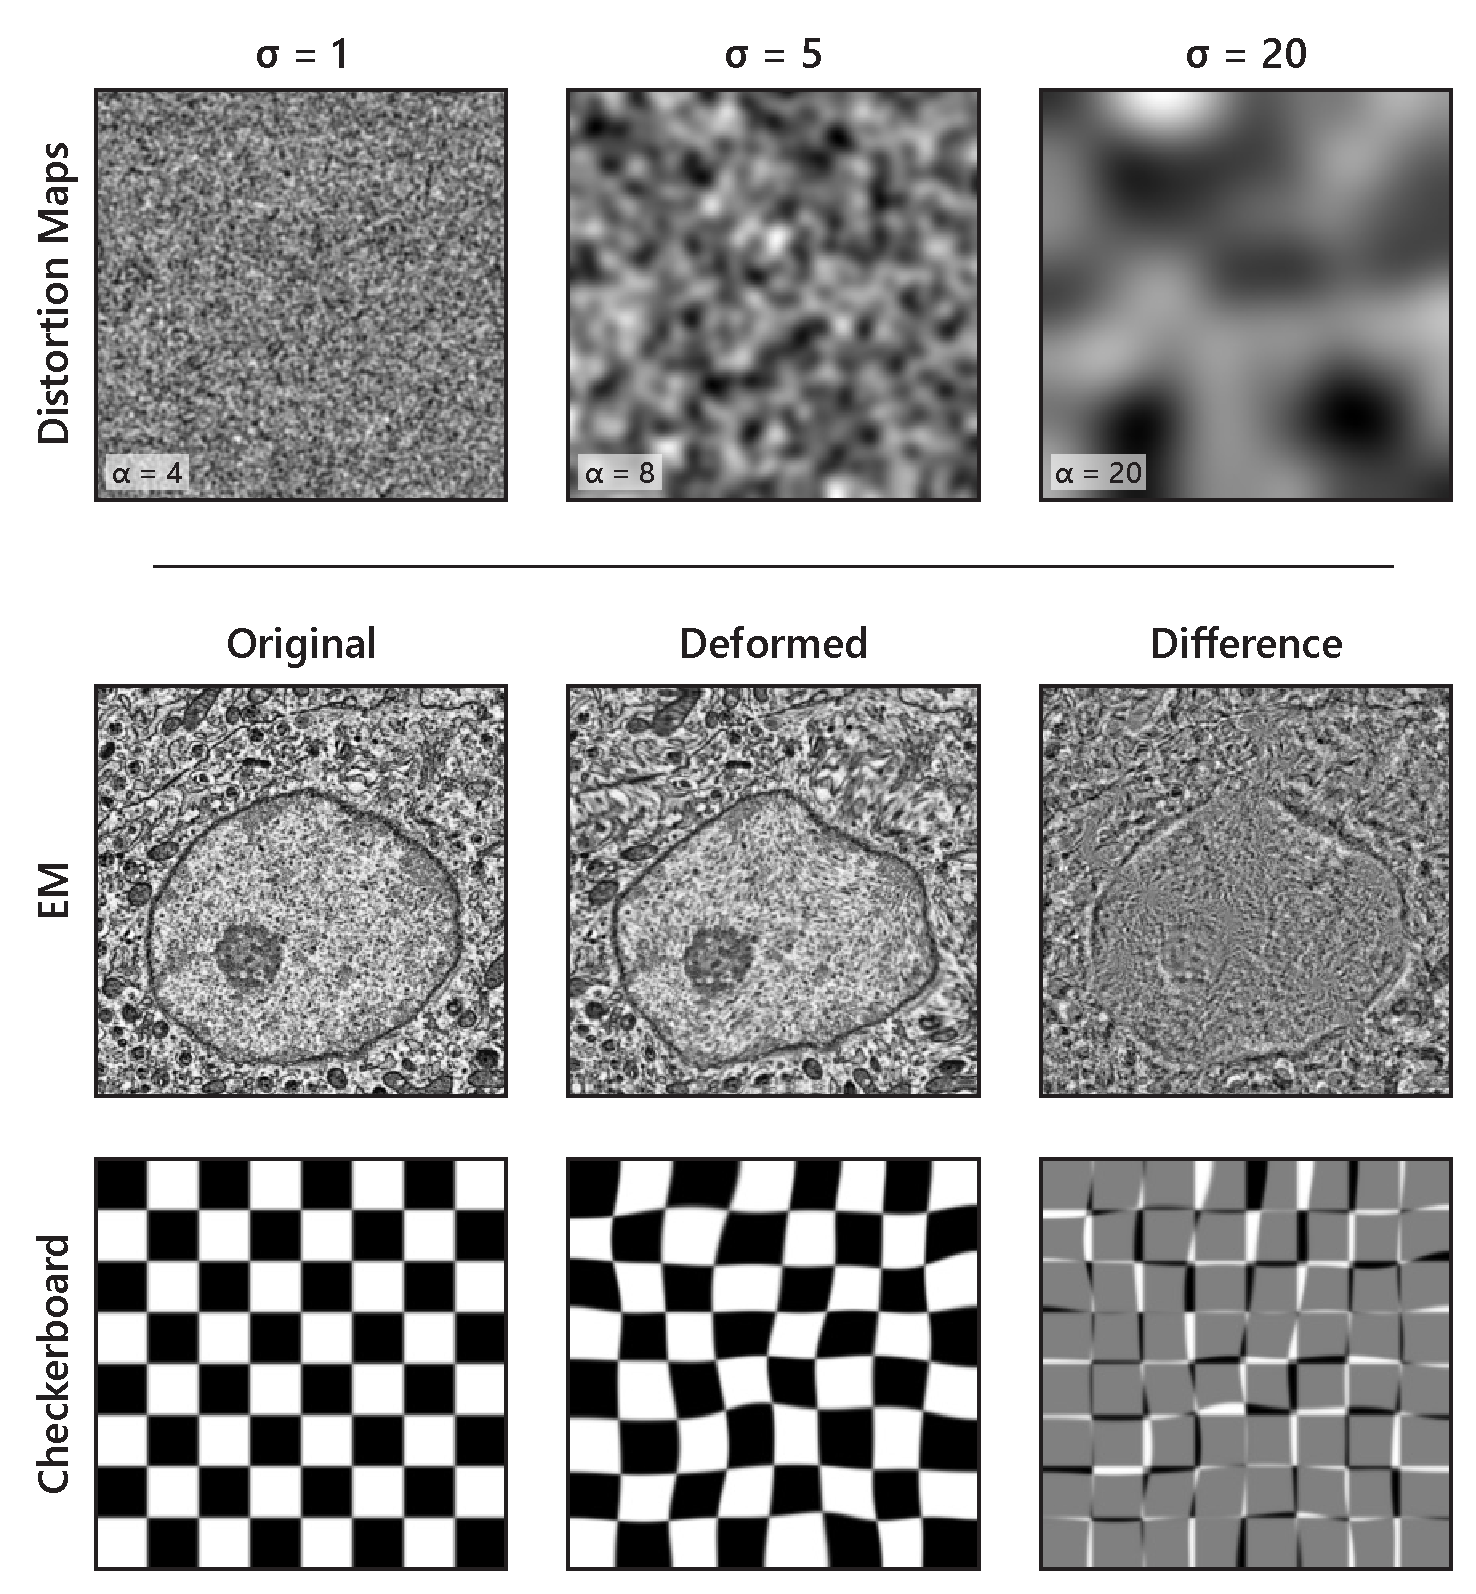
\includegraphics[width=\linewidth]{chapter-4/figures_PDF/fig4-M3_elastic.pdf}
    \caption{%
    Top: Distortion maps used for applying elastic deformations to training data. For small $\sigma$ the deformation resembles the addition of white noise, while for large $\sigma$ the deformation is more severe.
    Bottom: Elastic deformation applied to an EM training image and a checkerboard pattern.}
    \label{fig:4M_elastic}
\end{figure}

% --- Brightness / contrast ---
\subsubsection{Brightness \& contrast variation}
To account for the expected variations to brightness and contrast in EM image data acquired across different samples, microscopes, imaging settings, (day of the week), etc. the brightness and contrast levels are given a random adjustment. The brightness is varied ${\pm}$20\% by adding a gray-level bias, while the contrast is adjusted in the range $(0.75 < \delta < 1.5)$ where the value of each pixel, $x$, is scaled by
%
\begin{equation}
    (x - \bar{x})\,\delta + \bar{x}
\end{equation}
%
where $\bar{x}$ is the average intensity of the whole image.

% --- Noise augmentation ---
\subsubsection{Noise augmentation}
There are multiple sources of noise in the SEM detection chain, each with their own statistical distribution. The dominant source of noise on a properly operating SEM is, however, typically Poisson (shot noise) as additional contributions from the detector, scanning electronics, etc. tend to be much smaller than the statistical noise inherent in the signal \cite{joy2008noise}. Training images are therefore augmented with shot noise to improve the model’s robustness with respect to low SNR images (Figure \ref{fig:4M_noise}). The probability that a random variable $X$ is equal to $k$ is given by
%
\begin{equation}
    P(X=k;\lambda) = \frac{\lambda^{k} e^{-\lambda}}{k!}
\end{equation}
%
where $\lambda$ is the expectation value of $X$ as well as its variance.

% Fig 4.M4 (noise)
% ----------------
\begin{figure}[!tbh]
    \centering
    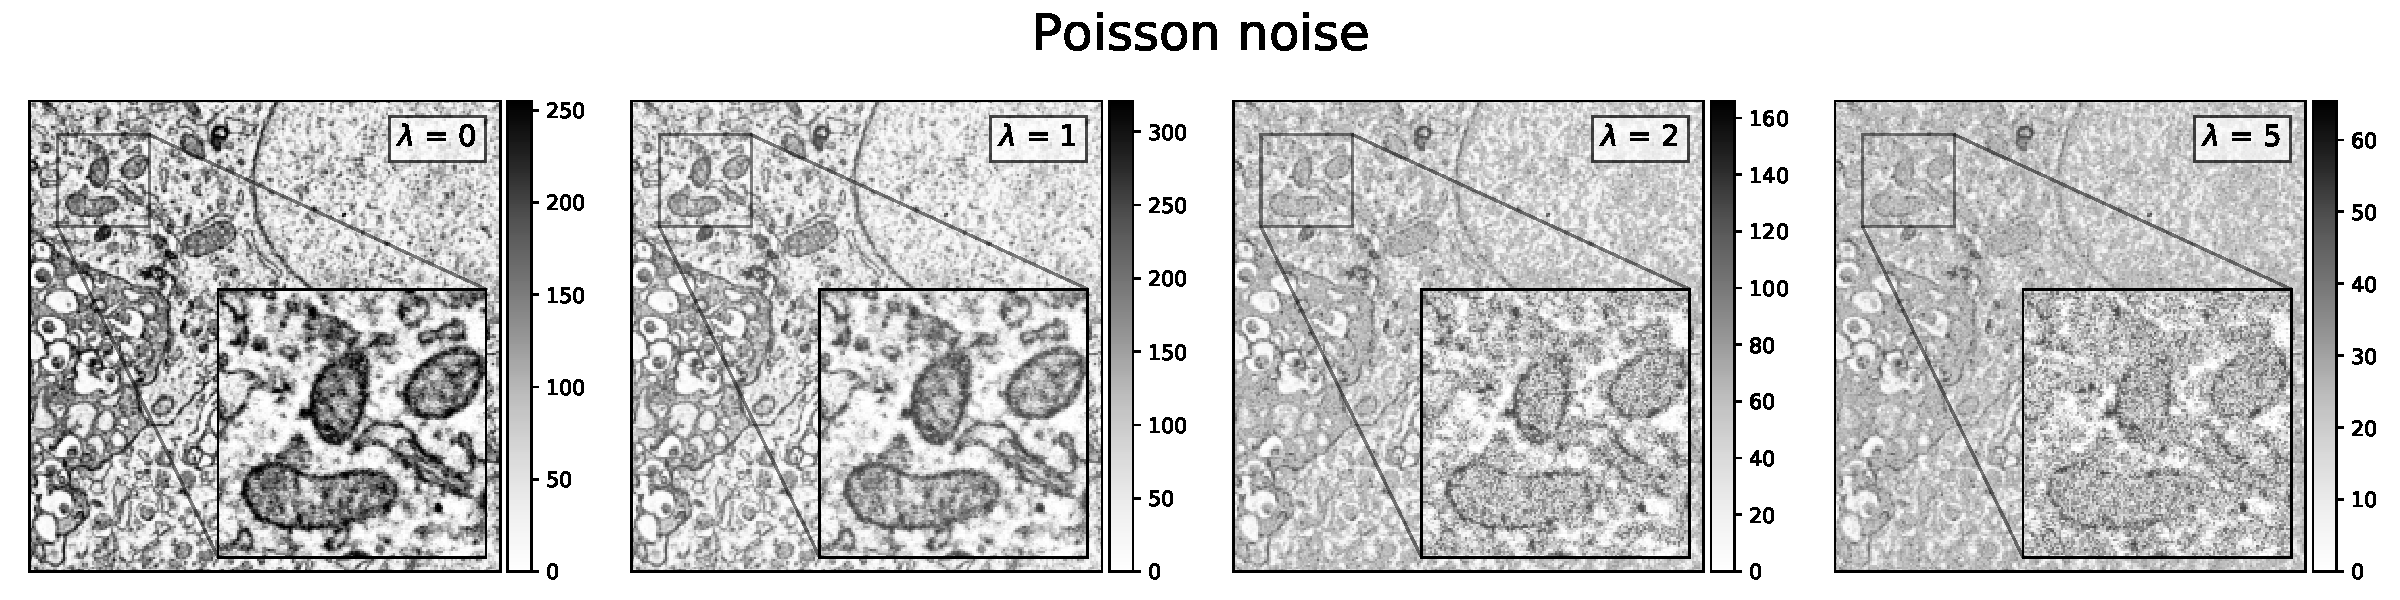
\includegraphics[width=\linewidth]{chapter-4/figures_PDF/fig4-M4_noise.pdf}
    \caption{Poisson noise added to an EM training image.
    Features become unrecognizable at high values of $\lambda$.}
    \label{fig:4M_noise}
\end{figure}


% 4.4.5
% -----
\subsection{Quantitative analysis}
\label{sec:4methods_analysis}

\subsubsection{Cell nuclei counting}
A combination of experts and trained volunteers were asked to recognize cell nuclei in datasets comprised of fluorescence signals obtained with a microscope and generated by CLEMnet. The experts consisted of two researchers from the University Medical Center Groningen who routinely examine islets of Langerhans, while the volunteers consisted of thirteen researchers from within the TU Delft Department of Imaging Physics who were trained to recognize cell nuclei in both FM and EM image data from comparable tissue. The annotations made by the experts were weighted by a factor 3.

An unsupervised, brute-force nearest neighbors search was used to filter outlier annotations from the EM dataset. For each annotated point, the Euclidean distance to every other annotated point was calculated. If a point was found to have at least 12 neighboring points (corresponding to ${\ge}$80\% of annotators) within a radius roughly equal to the average radius of a cell nucleus, the point was kept. Points with an insufficient amount of neighboring points were discarded, resulting in clusters of point clouds corresponding to the ground truth nuclei. $k$-means clustering was then used to agglomerate point clouds from which the centroid of each cluster could be computed and added to the ground truth set.

\subsubsection{Segmentation evaluation}
Segmentation performance is evaluated by the intersection over union (IoU), a similarity coefficient used to measure the overlap of two sets $A$ and $B$.
%
\begin{equation}
    IoU(A, B) = \frac{\left|\,A \cap B\,\right|}{\left|\,A \cup B\,\right|}
\end{equation}



% 4.4.6
% -----
\subsection{Segmentation}
\label{sec:4methods_segmentation}

\subsubsection{Fully supervised segmentation}

Segmentation masks for training were generated either by manually tracing cell nuclei in EM images of rat pancreas islets (using GIMP) or by thresholding the measured fluorescence or CLEMnet prediction images. A value of 0.2 was empirically chosen to be the threshold after rescaling the intensity range from (0, 255) to (0, 1). To reduce the burden on manual tracing, a higher zoom level was chosen than for generating fluorescence predictions. 96 images from across six different sections were manually segmented. One section was set aside for testing, while the five remaining sections were divided 80\%/20\% for training and validation. Implementation of the ResNet-34 model architecture was facilitated by Segmentation Models \cite{Yakubovskiy:2019}, which provides neural network frameworks for image segmentation compatible with Keras and Tensorflow.


\subsubsection{Partial points annotation}

Labelled images are generated in a two-phase process adapted from \textcite{qu2020weakly}. In the first phase (Figure \ref{fig:5M_segmentation}A), partial points annotation is used to generate a probability map for the location of cell nuclei. Partial points annotation was performed on the same dataset as used for the fully supervised segmentation. Though all nuclei visible in the EM were annotated, only five were chosen at random for generating Gaussian masks (PP Mask). The values for the Gaussian masks are given by
%
\begin{equation}
    M_i = 
    \begin{cases}
        \text{exp}\left({-\frac{D_i^2}{2\sigma^2}}\right) & \text{if}\; D_i < r_1, \\
        0 & \text{if}\; r_1 < D_i < r_2, \\
        -1 & \text{otherwise}
    \end{cases}
\end{equation}
%
where $D_i$ is the radial distance from each pixel $i$ to the nearest partial point, $\sigma$ is the standard deviation of the Gaussian distribution over each partial point, and $r_1$ and $r_2$ are the typical nuclear radius (estimated from the validation dataset) and the outer radius of background labels, respectively. Here we have used $r_1=\text{\SI{5}{\micro\meter}}$, $r_2 = 2 r_1$, and $\sigma = r_1 / 2$. In this way each pixel is classified as either nucleus ($>\text{0}$), background (0), or remains unlabelled ($-\text{1}$).

When trained on pairs of EM images and PP masks, ResNet-34 yields probability maps of predicted nuclei locations for given input EM test images. The initial probability map, though rather crude, is used to refine the PP mask to generate a better estimate of the background. The background estimate is updated according to the conditions
%
\begin{equation}
    M^N_i = 
    \begin{cases}
        M_i & \text{if}\; D_i < r_2, \\
        0 & \text{if}\; D_i > r_2 \quad \text{and} \quad p_i < 0.1, \\
        -1 & \text{otherwise}
    \end{cases}
\end{equation}
%
where $p_i$ is the probability of that pixel belonging to the nucleus class after iteration $N$. The pipeline is designed in such a way to as to iteratively yield better and better probability maps. We find, however, that the maps tend to converge after $N=\text{2}$ for this particular dataset.

% Fig 4.M5 (segmentation)
% -----------------------
\begin{figure}[!tb]
    \centering
    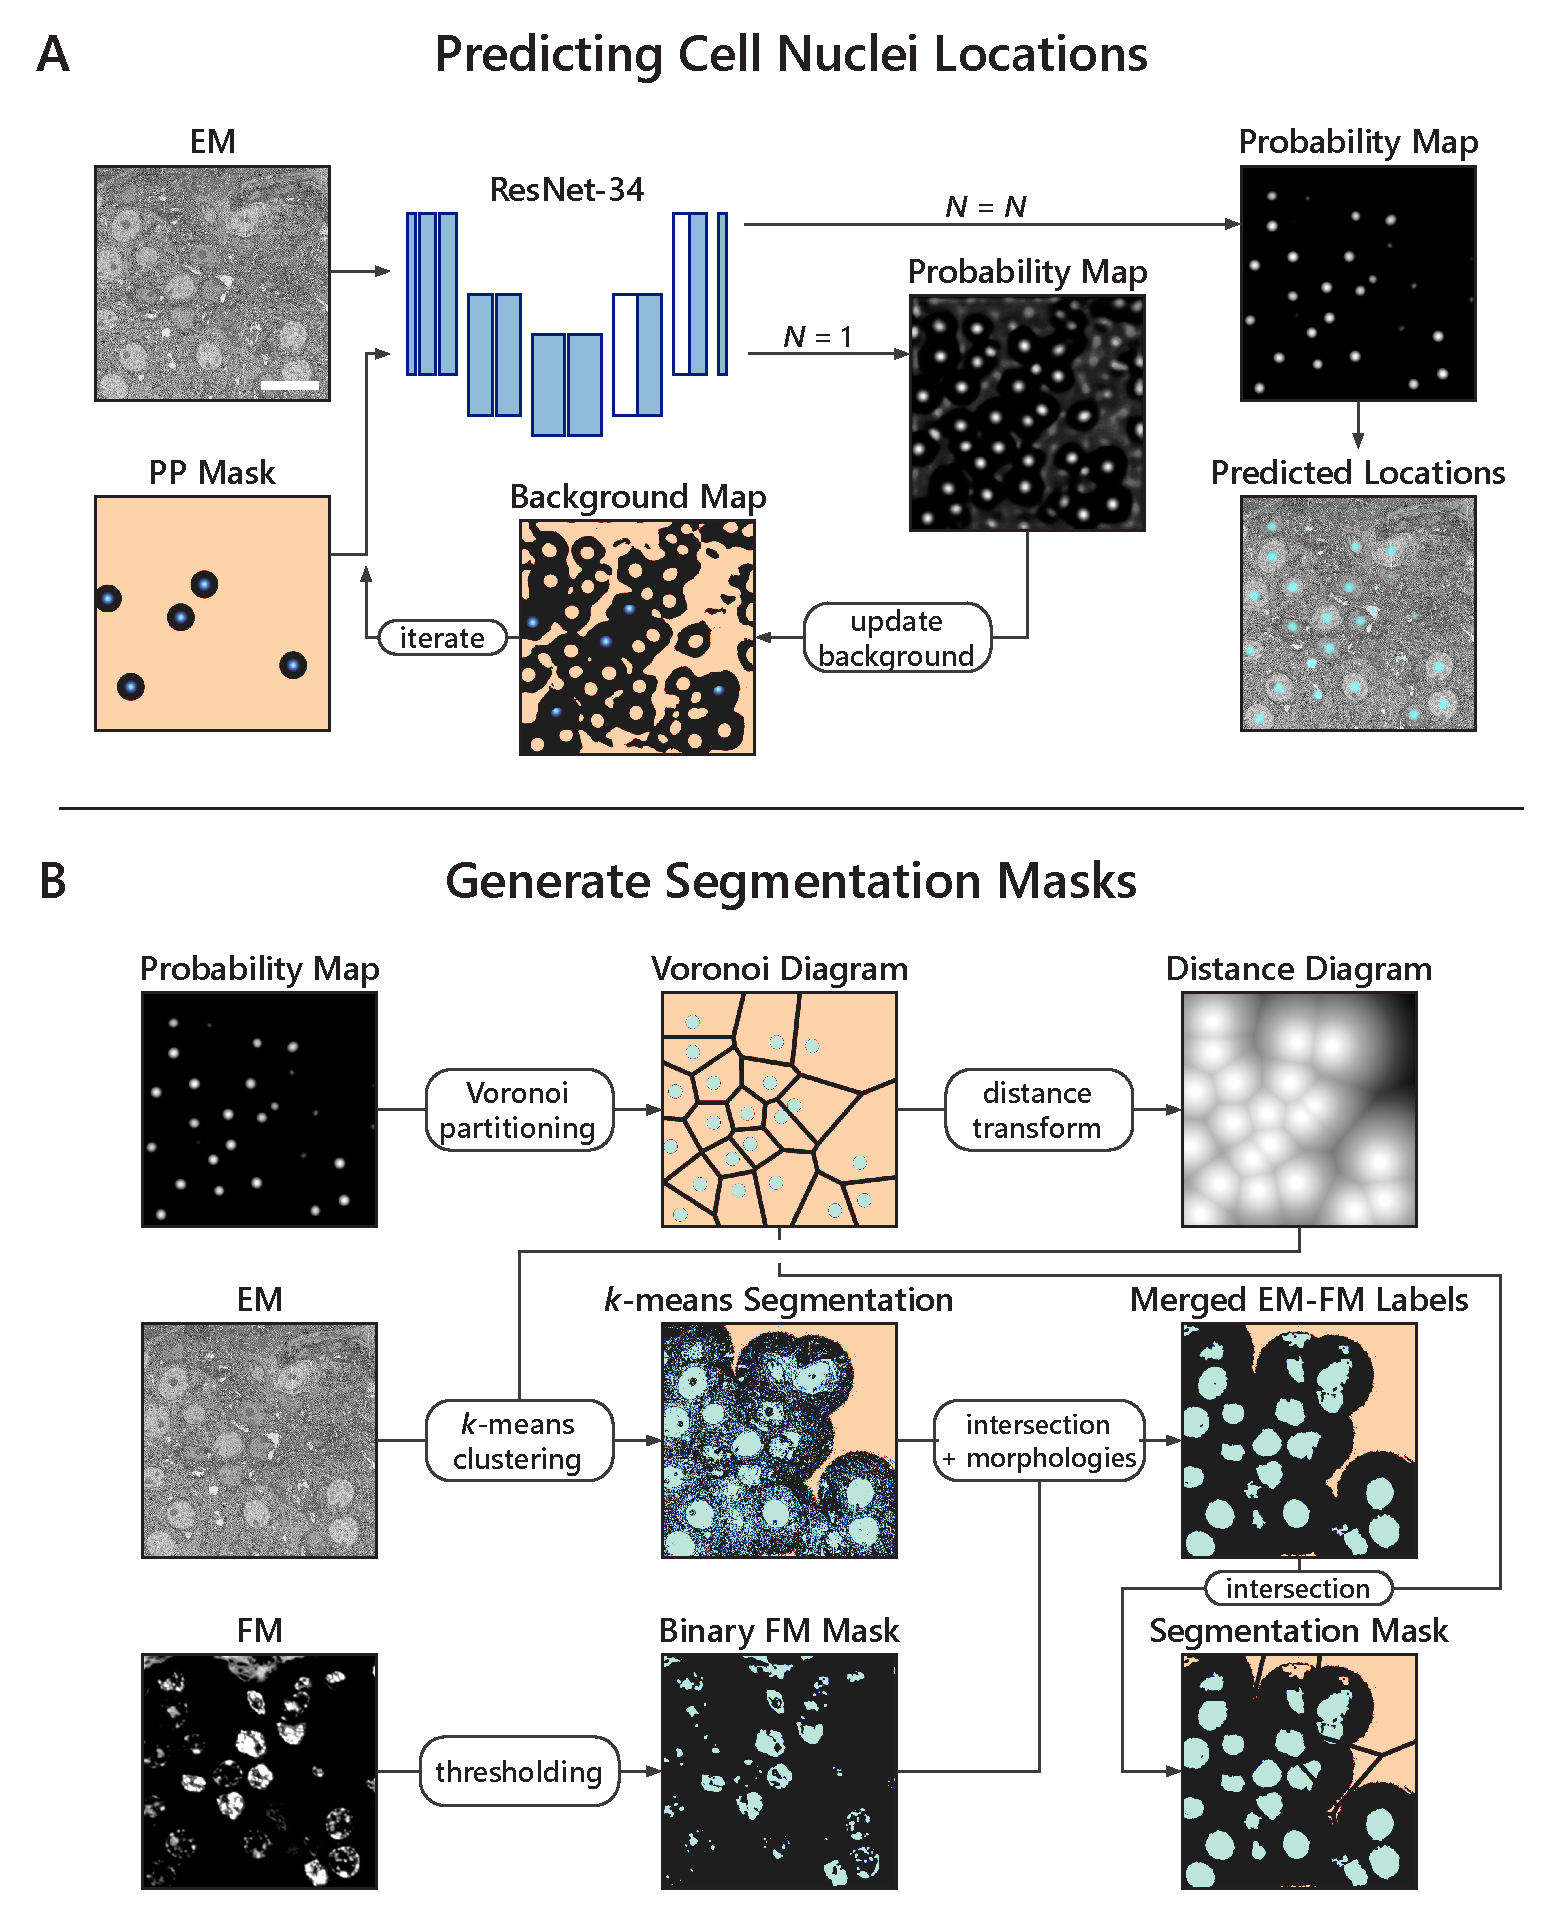
\includegraphics[width=0.95\linewidth]{chapter-4/figures_PDF/fig4-M5_segmentation.pdf}
    \caption{Semi-automated image processing pipeline for generating segmentation masks from partial points annotation.
    (A) Partial points annotation is used to create Gaussian mask images to train an instance of ResNet-34 to predict nuclei locations. The predictions are refined through self-training to yield more accurate probability masks.
    (B) A Voronoi diagram based off of the probability map in (A) is merged with labelled images from $k$-means clustering to create segmentation masks for training a separate instance of ResNet-34 for organelle segmentation.
    Legend: white (or cyan) -- nucleus; black -- background; beige -- unlabelled.
    Scale bar: (A) \SI{10}{\micro\meter} (scale bar in EM applies to all images).}
    \label{fig:5M_segmentation}
\end{figure}

In phase two (Figure \ref{fig:5M_segmentation}B), segmentation masks are generated by a combination of $k$-means clustering and a Voronoi partitioning of the nuclei detected in phase one. These two labelling schemes are complementary to one another. $k$-means clustering preserves the spatial information in the EM image, providing the contour of the nuclei at the expense of having greater uncertainty, while the Voronoi partition provides accurate nuclei localization at the expense of underestimating the background label. The EM image is multiplied by the distance transform of the Voronoi diagram prior to $k$-means clustering to amplify nuclei. Clustering is then done with $k=\text{3}$. We choose to subtract a value of 1 from the resulting image such that the background goes to $-\text{1}$ (unlabelled). In this way the model does not train on regions of the image where a label cannot easily be inferred from either the $k$-means clustering or Voronoi partitioning. These regions are typically in the void between adjacent nuclei where it can be disadvantageous to make an assumption on whether a pixel belongs to the nucleus or background class, as it is possible that a nucleus was missed in phase one.

The fluorescence image is independently thresholded and intersected with the $k$-means clustered image. Small segments are removed via morphological opening, closing, and erosion operations. Larger segments are filtered by convexity, measured as the ratio of the area of each segment relative to the area of its convex hull. Segments with convexity less than 0.85 become unlabelled. Lastly, the merged labels from $k$-means clustering of the EM and thresholding of the FM are intersected with the Voronoi diagram to result in a final segmentation mask. Pairs of segmentation masks and EM images are then used to train an instance of ResNet-34 for organelle segmentation in the same manner as was described for fully supervised segmentation. Note that the fluorescence image was originally included as a separate channel during $k$-means clustering, but the results from doing so were marginally worse: final IoU score of 67\% vs 72\%.
